\documentclass[12pt, a4paper]{article}
\usepackage[a4paper,top=1.5cm, bottom=1.5cm, left=2cm, right=2cm]{geometry}
\usepackage{graphicx} % Required for inserting images
%%% Работа с русским языком
\usepackage{cmap}					% поиск в PDF
\usepackage{mathtext} 				% русские буквы в фомулах
\usepackage[T2A]{fontenc}			% кодировка
\usepackage[utf8]{inputenc}			% кодировка исходного текста
\usepackage[english,russian]{babel}	% локализация и переносы
\usepackage{float}
\usepackage{subcaption}
\usepackage{wrapfig}
\usepackage{tabularx}
\usepackage{multirow}

\usepackage[unicode, colorlinks=true, urlcolor=blue]{hyperref}
\usepackage[rgb]{xcolor}
\hypersetup{
colorlinks=true,urlcolor=blue
}
%%% Дополнительная работа с математикой
\usepackage{amsmath,amsfonts,amssymb,amsthm,mathtools} % AMS
\usepackage{icomma} % "Умная" запятая: $0,2$ --- число, $0, 2$ --- перечисление
%% Номера формул
\mathtoolsset{showonlyrefs=true} % Показывать номера только у тех формул, на которые есть \eqref{} в тексте.
%% Шрифты
\usepackage{euscript}	 % Шрифт Евклид
\usepackage{mathrsfs} % Красивый матшрифт
%% Свои команды
\DeclareMathOperator{\sgn}{\mathop{sgn}}
%% Перенос знаков в формулах (по Львовскому)
\newcommand*{\hm}[1]{#1\nobreak\discretionary{}
{\hbox{$\mathsurround=0pt #1$}}{}}


\usepackage{indentfirst}
\usepackage{amsmath,amssymb}
\usepackage[italicdiff]{physics}
\graphicspath{{images/}}
\DeclareGraphicsExtensions{.pdf,.png,.jpg}
\usepackage{enumitem}
\usepackage{caption}
\usepackage{array}
\usepackage{ragged2e}







\begin{document}



\include{titlepage}
\begin{titlepage}
\thispagestyle{empty}

\begin{center}
\small
Министерство науки и высшего образования Российской Федерации\\[2mm]
\textbf{ФЕДЕРАЛЬНОЕ ГОСУДАРСТВЕННОЕ АВТОНОМНОЕ
ОБРАЗОВАТЕЛЬНОЕ УЧРЕЖДЕНИЕ ВЫСШЕГО ОБРАЗОВАНИЯ}\\[1mm]
«МОСКОВСКИЙ ФИЗИКО-ТЕХНИЧЕСКИЙ ИНСТИТУТ\\
(НАЦИОНАЛЬНЫЙ ИССЛЕДОВАТЕЛЬСКИЙ УНИВЕРСИТЕТ)»\\
(МФТИ, Физтех)
\end{center}

\vspace{18mm}

\begin{center}
\large \textbf{КАФЕДРА ЭЛЕКТРОНИКИ}\\[10mm]
\Large \textbf{ОТЧЁТ}\\[2mm]
\large \textbf{ПО ЛАБОРАТОРНОЙ РАБОТЕ}\\[14mm]
\Large \textbf{КОНВЕКТИВНАЯ ДИФФУЗИЯ В МОЛЕКУЛЯРНО-ЭЛЕКТРОННЫХ ПРЕОБРАЗОВАТЕЛЯХ}
\end{center}

\vfill

% Блоки с подписями слева, линии и пояснения справа
\noindent
\begin{tabular}{@{}p{0.44\linewidth}p{0.52\linewidth}@{}}
\textit{Работу выполнили:} & Рагозина Елизавета,

Струков Олег,

Топольский Михаил,

Группа Б04-404 \\[8mm]

\textit{Работу принял, оценка:} & \\[3mm]
 \\
\end{tabular}


\vspace{12mm}

\begin{center}
\small Долгопрудный, \the\year{}~г.
\end{center}

\end{titlepage}




\newpage
\pagenumbering{arabic}

\textbf{Цель работы}: Исследование процессов протекания тока в молекулярно-электронном преобразователе в стационарных и нестационарных условиях. 

\textbf{Оборудование и ПО}: Для задания входных сигналов и регистрации  полученных данных 
используется программа calib для управления многофункциональным модулем ЦАП/АЦП. Обработка данных осуществляется с помощью пакета Dadisp. 

\section*{Введение}

Системы на основе явления конвективной диффузии в растворах электролитов представляют собой перспективную технологию для измерения параметров движения и волновых полей. В данных устройствах жидкость выступает в роли инерционной массы и преобразующего элемента, что исключает наличие элементов точной механики. Принцип действия заключается в модуляции электрического тока за счёт перемещения активных носителей заряда под воздействием внешнего механического сигнала. Высокий коэффициент преобразования обеспечивает чувствительность, превышающую показатели электродинамических систем, что делает их пригодными для регистрации колебаний малой амплитуды. Коэффициент преобразования механического возмущения в электрический ток при этом достигает $1\,\frac{\text{А}}{\text{м/с}}$.

Наибольшее распространение имеют молекулярно-электронные преобразователи (МЭП), выполненные на базе двух электрохимических ячеек (ЭЯ), включенных по дифференциальной схеме. Принципиальная схема такого преобразователя показана на рис. 1. 

% \begin{justify}
% Уникальной и перспективной технологией для измерения параметров движения и волновых полей являются системы, построенные на основе явления конвективной диффузии в растворах электролитов. Они не содержат элементов точной механики, а в качестве инерционной массы и преобразующего элемента внешнего воздействия в электрический ток используется жидкость, которая, подобно <<электронному газу>> в вакуумных приборах, осуществляет перенос активных носителей заряда, 
% промодулированный внешним механическим сигналом. Основная физическая идея подобного устройства позаимствована из вакуумной электроники. В самом деле, увеличение тока в вакуумном триоде можно осуществить не только изменением сеточного напряжения, но также и простым перемещением сетки, например под действием внешнего механического сигнала.
% \par
% В то время как создать подобный преобразователь механического 
% воздействия на базе вакуумного триода технически крайне сложно, данная идея осуществима в системах на основе проводящей жидкости. 
% \par
% Если на электроды подана разность потенциалов, то между анодом и катодом устанавливается стационарное распределение концентрации активных носителей заряда, ведущее к возникновению постоянного электрического тока, пропорционального градиенту концентрации на электродах. При воздействии внешнего сигнала происходит перемещение рабочей жидкости и увлечение ею активных ионов, которое ведет к изменению их концентрации на электродах. Соответственно во внешней цепи происходят вариации тока. При этом подобно тому, как это происходит в вакуумном триоде, осуществляется усиление сигнала по мощности за счёт использования энергии внешнего источника. Коэффициент преобразования механического возмущения в электрический ток при этом достигает $1\,\frac{\text{А}}{\text{м/с}}$, что существенно превышает чувствительность электродинамических систем, широко распространенных в сейсмологии в настоящее время, и делает электрохимические преобразователи пригодными для регистрации удаленных землетрясений и прочих колебаний малой амплитуды.
% \end{justify}
\begin{figure}[H]
	\centering
	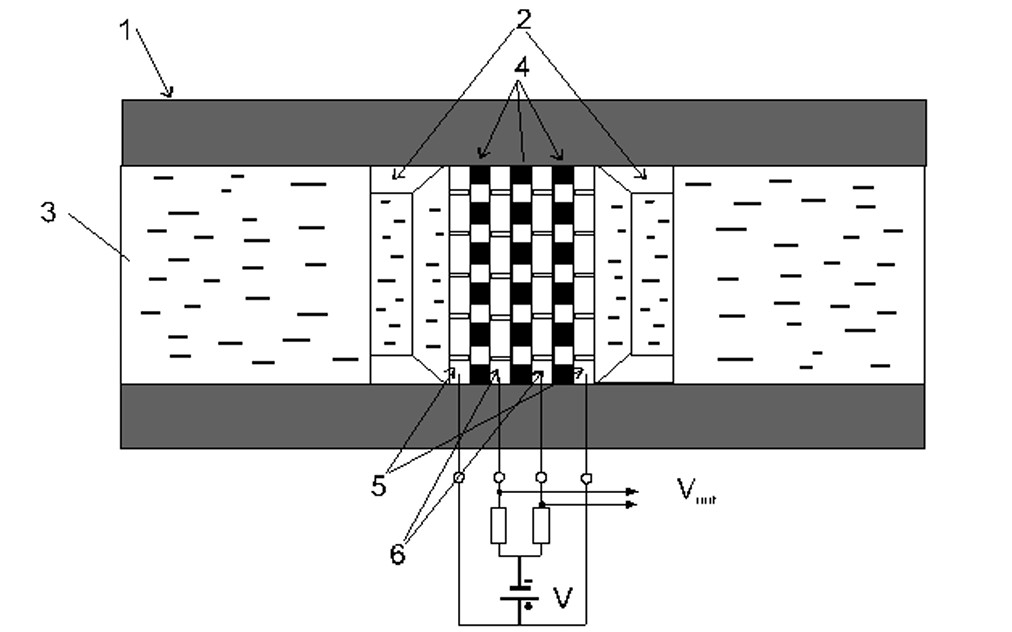
\includegraphics[width=0.9\linewidth]{p1.jpg}
	\caption{Молекулярно-электронный преобразователь}
	% \label{pic_3}
\end{figure}


Конструкция устройства включает следующие основные элементы:
\begin{itemize}[label=--]
    \item \textbf{Диэлектрическая трубка} (1);
    \item \textbf{Электродный узел} (2), помещённый внутрь трубки;
    \item \textbf{Раствор электролита} (3), заполняющий внутренний объем;
    \item \textbf{Плоские сетчатые электроды}, установленные внутри узла:
    \begin{itemize}
        \item аноды (5);
        \item катоды (6);
    \end{itemize}
    \item \textbf{Пористые перегородки} (4), разделяющие электроды.
\end{itemize}
В МЭП могут быть использованы различные окислительно-восстановительные реакции, например: йод - йодид, ферро - феррицианид и др. При этом чаще всего электроды ЭЯ изготавливаются из металла, который не участвует в обмене катионами, а осуществляет только электронный обмен.

В настоящее время наиболее широкое применение получили йод-йодидные системы с платиновыми электродами [1, 4]. Электролит такой системы состоит из водного раствора йодида калия $KI$ и йода $I_2$. В избытке йодида йод переходит в хорошо растворимое комплексное соединение - трийодид по следующей схеме:
\[
I_2 + I^- \rightarrow I_3^-.
\]
При прохождении тока через МЭЯ на катодах происходит восстановление йода:
\[
I_3^- + 2e \rightarrow 3I^-;
\]
а на аноде окисление йода:
\[
3I^- - 2e \rightarrow I_3^-.
\]
Ионы калия не принимают участия в реакциях.
\par

Электрический ток, проходящий через ЭЯ, определяется как концентрацией ионов, так и механизмом их движения в растворах электролитов. Перенос заряда в жидкости можно разделить на три независимых механизма: миграция, диффузия и конвекция, каждый из них в определенных физико-химических процессах играет главную роль.

\par

Математическая формулировка задачи для расчёта тока, текущего через электрохимическую ячейку, сводится к решению уравнений гидродинамики и диффузии:
\begin{align}
    \frac{\partial \mathbf{v}}{\partial t} + (\mathbf{v}\nabla)\mathbf{v} &= -\frac{\nabla p}{\rho} + \nu\Delta\mathbf{v} + \label{eq:1} \\
    \operatorname{div} \mathbf{v} &= 0 \label{eq:2} \\
    \frac{\partial n}{\partial t} &= D\Delta n + (\mathbf{v}, \nabla)n + \label{eq:3}
\end{align}
где $\mathbf{v}$ -- скорость электролита, $p$ -- давление, $\rho$ -- плотность электролита, $\nu$ -- вязкость жидкости, $n$ -- концентрация носителей тока (ионов трийодида), $D$ -- коэффициент их диффузии, $j$ -- плотность потока. В системе с плоскими электродами эти уравнения фактически являются одномерными.

В качестве граничных условий к уравнениям (3) - (4) используются следующие соотношения:
\begin{enumerate}
    \item Отсутствие потока активных ионов через диэлектрические поверхности.
    \item Уравнения, определяющие скорости электрохимических реакций в зависимости от концентрации ионов и скачка потенциала на границе электрод/электролит. Получение таких уравнений является предметом отдельной области исследований -- электродной кинетики.
\end{enumerate}

Кроме того, дополнительно накладывается интегральное соотношение, выражающее закон сохранения количества активных ионов
\begin{equation}
\iiint n(x, y, z, t) dV = V n_0, \tag{4}
\end{equation}
где $V$ -- объем электролита, $n_0$ -- равновесная концентрация.

Следует отметить, что система уравнений (1) - (3) является приближённой и не учитывает наличие в МЭЯ электрического поля и объемного заряда, которые могут влиять на гидродинамическое движение раствора и конвективный перенос ионов.

Ниже будут рассмотрены решения уравнения (1) -- (3) в некоторых частных случаях, представляющих практический интерес.

\section*{Стационарный случай}

Величина диффузионного тока, текущего через электрод:
\[
I_D = -eSD\nabla n
\]

В стационарном случае уравнение диффузии (3) будет иметь вид:

\[
\Delta n = 0.
\]

Выражение для тока, текущего через 
катод или анод: 

\begin{equation}
I_D = -\frac{e S D n_0}{d} \, \mathrm{th}\!\left( \frac{e U}{2 k_\mathrm{B} T} \right).
\label{eq:diode_current}
\end{equation}

Соответствующая вольт-амперная характеристика представлена на 
рисунке:

\begin{figure}[H]
	\centering
	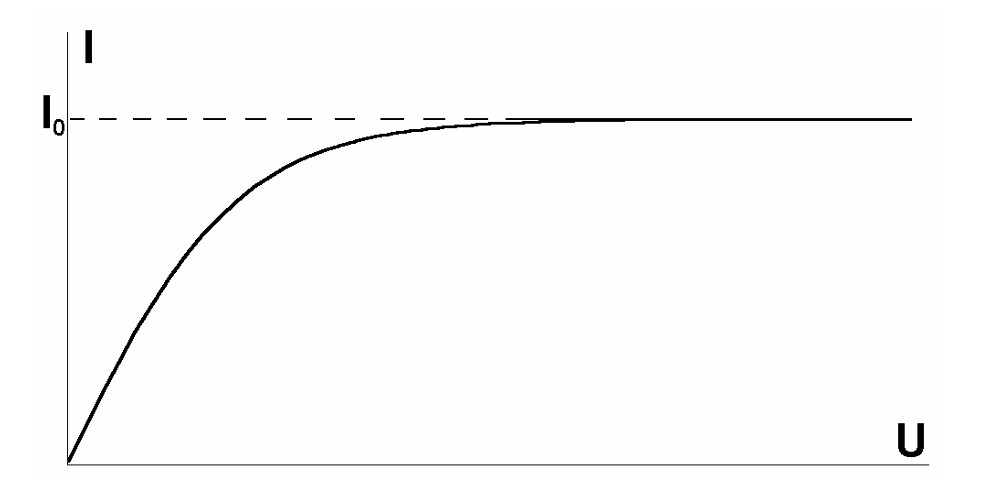
\includegraphics[width=0.7\linewidth]{p2.jpg}
	\caption{ВАХ молекулярно-электронной ячейки с неподвижным электролитом}
	% \label{pic_3}
\end{figure}

\section*{Конвективная диффузия}

Если жидкость в МЭЯ приходит в движение под действием каких-либо внешних сил, то, наряду с диффузионным, появляется также конвективный ток, обусловленный увлечением ионов движущейся жидкостью. В линейном приближении конвективный ток пропорционален скорости движущейся жидкости $V$ и определяется соотношением:
\begin{equation}
I_k = e S n V.
\label{eq:convective_current}
\end{equation}

Полезно сравнить, при каких минимальных скоростях движения жидкости конвективный ток становится сравнимым с диффузионным. Для оценок положим расстояние между электродами $d \approx 10^{-2}\,\text{см}$, $D = 10^{-5}\,\text{см$^2$/с}$ получаем $I_D \approx I_k$ при $V \approx 10^{-3}\,\text{см/с}$. Это означает, что столь малое значение скорости движения жидкости способно изменить ток в цепи МЭЯ на величину, сравнимую с ним самой. Именно этим объясняется высокая чувствительность молекулярно-электронных преобразователей к действию внешних механических возмущений.

В основе работы МЭЯ лежит конвективная диффузия, вызванная действием внешних механических возмущений. 

Найдём изменение тока через молекулярно-электронный преобразователь, вызванное протеканием электролита. В случае малых изменений механических величин можно ограничиться линейным приближением. В этом приближении введём для удобства новую переменную $c(x,t)$, которая определяется из выражения
\begin{equation}
n = n_0 \left( 1 - \frac{x}{d} \, \mathrm{th}\!\left( \frac{eU}{2k_\mathrm{B}T} \right) \right) + c(x,t).
\label{eq:carrier_concentration_perturbation}
\end{equation}

В этом случае уравнение конвективной диффузии перепишем:

\begin{equation}
\frac{\partial c}{\partial t} - D \frac{\partial^2 c}{\partial x^2} = V_0 e^{i\omega t} \, \frac{n_0}{d} \, \mathrm{th}\!\left( \frac{eU}{2k_\mathrm{B}T} \right).
\label{eq:diffusion_perturbation_equation}
\end{equation}

Решение:

\begin{equation}
X(x) = A_1 e^{(1+i)\sqrt{\frac{\omega}{2D}}\,x} + A_2 e^{-(1+i)\sqrt{\frac{\omega}{2D}}\,x} - \frac{i V_0 n_0}{d \omega} \, \mathrm{th}\!\left( \frac{eU}{2k_\mathrm{B}T} \right).
\label{eq:solution_X_x}
\end{equation}

Для определения постоянных воспользуемся граничными условиями и получим:

\begin{equation}
X(d) = X(-d) = 0.
\label{eq:boundary_conditions_X}
\end{equation}

В результате получим:
\begin{equation}
A_1 = A_2 = i \, \frac{V_0 n_0}{2 d \omega} \, \frac{\mathrm{th}\!\left( \dfrac{eU}{2k_\mathrm{B}T} \right)}{\ch\!\left( (1+i)\sqrt{\dfrac{\omega}{2D}}\, d \right)}.
\label{eq:A1_A2_solution}
\end{equation}

Окончательно, для концентрации $c(x,t)$ имеем
\begin{equation}
c(x,t) = i \, \frac{V_0 n_0}{d \omega} \, \mathrm{th}\!\left( \frac{eU}{2k_\mathrm{B}T} \right) e^{i\omega t} \left( \frac{ \ch\!\left( (1+i)\sqrt{\dfrac{\omega}{2D}}\, x \right) }{ \ch\!\left( (1+i)\sqrt{\dfrac{\omega}{2D}}\, d \right) } - 1 \right).
\label{eq:concentration_final}
\end{equation}

Выражение для полного тока, те
кущего через систему:

\begin{equation}
I = -\frac{e S D n_0}{d} \, \mathrm{th}\!\left( \frac{eU}{2k_\mathrm{B}T} \right) \left[ 1 - e^{i\omega t}(1 - i) \sqrt{\frac{1}{2\omega D}} \, V_0 \, t h\!\left( (1 + i) \sqrt{\frac{\omega}{2D}} \, d \right) \right].
\label{eq:current_full_expression}
\end{equation}


\begin{figure}[H]
	\centering
	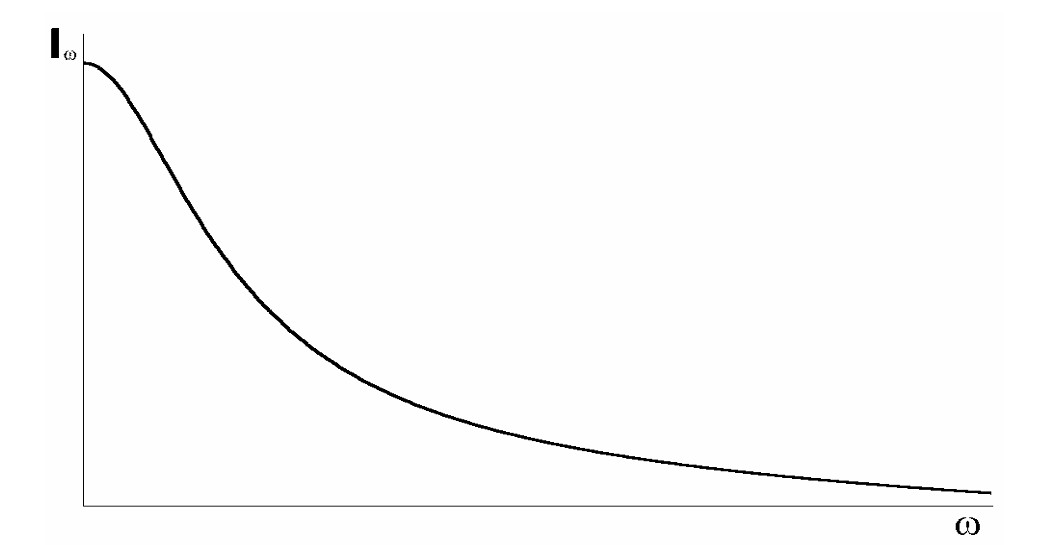
\includegraphics[width=0.8\linewidth]{p3.jpg}
	\caption{Зависимость модуля выходного тока МЭЯ от частоты в условиях 
конвективной диффузии }
	% \label{pic_3}
\end{figure}

\section*{Методика эксперимента}

Для стационарного случая проводится измерение ВАХ, т.е. зависимости выходного тока ЭЯ в условиях стационарной диффузии от приложенной к электродам разности потенциалов.
\par

На рисунке приведена схема устройства:

\begin{figure}[H]
	\centering
	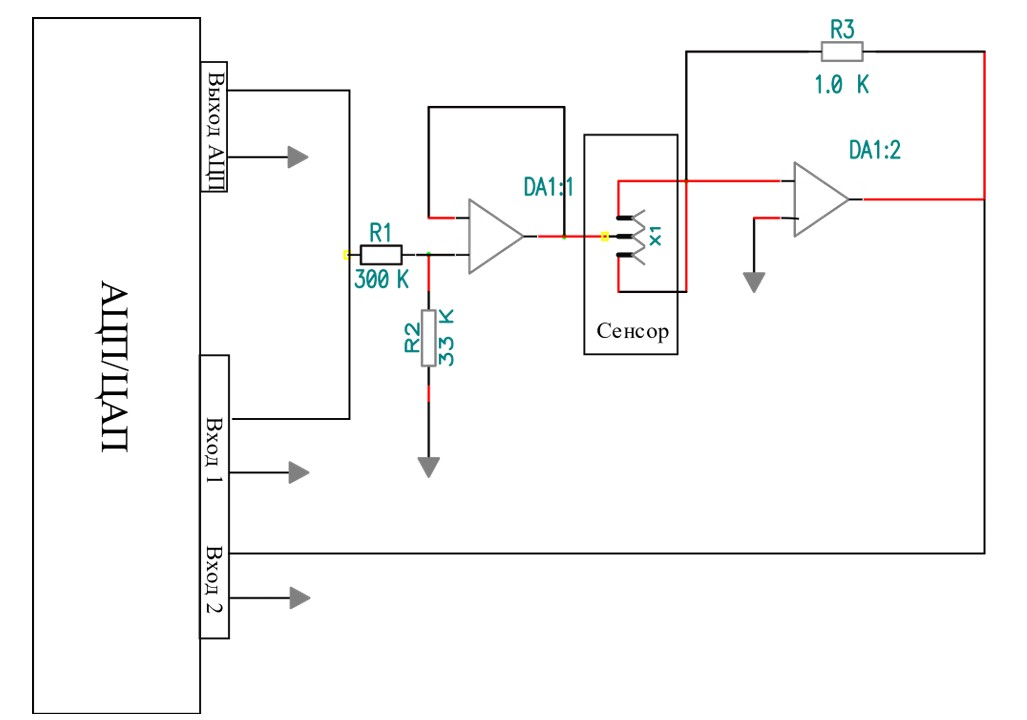
\includegraphics[width=0.8\linewidth]{p4.jpg}
	\caption{Принципиальная схема экспериментальной установки для измерения стационарной ВАХ}
	% \label{pic_3}
\end{figure}






\section*{Ход работы}

Была снята ВАХ прибора, результаты представлены в таблице:

\begin{table}[H]
\centering
\begin{tabular}{|c|c|c|c|c|c|c|c|c|c|c|}
\hline
$U_{\text{а-к}}$, мВ & 2    & 5    & 10  & 15  & 20    & 30    & 40   & 50   & 100  & 150  \\ \hline
$U_{\text{ЦАП}}$, мВ & -47  & -51  & -56 & -61 & -66,5 & -76,5 & -86  & -96  & -146 & -196 \\ \hline
$U_{\text{АЦП}}$, мВ & -40  & -11  & 25  & 63  & 101   & 160   & 225  & 270  & 496  & 670  \\ \hline
I, мкА & -4,0 & -1,1 & 2,5 & 6,3 & 10,1  & 16,0  & 22,5 & 27,0 & 49,6 & 67,0 \\ \hline
\end{tabular}
\caption{Вольт-амперная характеристика}
\label{tab:measurements}
\end{table}

Построен график полученной зависимости:
\begin{figure}[H]
	\centering
	
\includegraphics[width=1\linewidth]{1.pdf}
	\caption{График зависимости $I(U)$}
\end{figure}

Из полученных измерений была оценена площадь электродов: 

\begin{equation}
I_0 = \frac{e S D n_0}{d} \qquad \Longrightarrow \qquad S = \frac{I_0 d}{e D n_0}.
\label{eq:area_from_current}
\end{equation}

При подстановке следующих значений величин
\begin{itemize}
    \item $I_0 \thicksim 100~\text{мкА} = 10^{-4}~\text{А}$;
    \item $d \approx 100~\text{мкм} = 10^{-4}~\text{м}$;
    \item $e = 1,602 \cdot 10^{-19}~\text{Кл}$;
    \item $D = 10^{-5}~\text{см$^2$/с} = 10^{-9}~\text{м$^2$/с}$;
    \item $n_0 \thicksim 10^{25}~\text{м$^{-3}$}$ 
\end{itemize}

Было оценено $S \thicksim 5 \text{ мм}^{2}$.


Далее была снята АЧХ системы:

\begin{table}[H]
\centering
\begin{tabular}{|c|c|c|c|c|c|c|c|c|}
\hline
Частота, Гц & 0,1  & 0,2   & 0,5   & 1     & 2     & 5    & 10   & 20    \\ \hline
Вход, $U_{max} - U_{min}$, мВ & 40   & 40    & 40    & 40    & 40    & 40   & 40   & 40    \\ \hline
Выход, $U_{max} - U_{min}$, мВ & 126  & 156,2 & 202,6 & 125   & 135   & 73,2 & 32,4 & 11    \\ \hline
Отношение $U_\text{вых}/U_\text{вх}$ & 3,15 & 3,905 & 5,065 & 3,125 & 3,375 & 1,83 & 0,81 & 0,275 \\ \hline
\end{tabular}
\caption{Амплитудно-частотная характеристика}
\end{table}

График зависимости представлен на рисунках 6 и 7:

\begin{figure}[H]
	\centering
	
\includegraphics[width=1\linewidth]{2.pdf}
	\caption{График зависимости $U_\text{вых}/U_\text{вх}(f)$}
\end{figure}

\begin{figure}[H]
	\centering
	
\includegraphics[width=1\linewidth]{3.pdf}
	\caption{График зависимости $U_\text{вых}/U_\text{вх}(f)$ в двойном логарифмическом масштабе}
\end{figure}


\section*{Вывод}
В ходе работы были исследованы процессы протекания тока в молекулярно-электронном преобразователе в стационарных и нестационарных условиях. Снята вольт-амперная характеристика электрохимической ячейки, по результатам которой оценена площадь электродов
($S \thicksim 5$ мм$^2$). Получена амплитудно-частотная характеристика системы, демонстрирующая зависимость коэффициента передачи от частоты внешнего механического возмущения. Экспериментальные данные подтверждают высокую чувствительность МЭП к малым механическим воздействиям за счёт явления конвективной диффузии в растворе электролита.


\end{document}